\documentclass[12pt, twoside]{article}
\usepackage{jmlda}
\newcommand{\hdir}{.}

% Здесь можно определять собственные команды, они будут действовать только внутри статьи:
\newenvironment{coderes}%
    {\medskip\tabcolsep=0pt\begin{tabular}{>{\small}l@{\quad}|@{\quad}l}}%
    {\end{tabular}\medskip}

\begin{document}

\title{Рекомендации по подготовке статей к публикации}
\author{Редколлегия журнала}
\email{info@jmlda.org}
\organization{ФИЦ <<Информатика и управление>> РАН, г.~Москва, ул.~Вавилова, 44/2}
\abstract{Данный документ содержит рекомендации по~подготовке статей в~издательской системе \LaTeXe\
    с~использованием стилевого файла \texttt{jmlda.sty}.}
\titleEng{Style guide for authors}
\authorEng{JMLDA editorial board}
\organizationEng{Federal Research Center ``Computer Science and Control'' of RAS, 44/2~Vavilova~st., Moscow, Russia}
\abstractEng{
    This document explains how to prepare papers using \LaTeXe\ typesetting system and \texttt{jmlda.sty} package.
}
\doi{10.21469/22233792}
\receivedRus{01.01.2017}
\receivedEng{January 01, 2017}

\maketitle
\linenumbers
\section{Введение}
Данный документ является примером статьи, изготовленной согласно представленным в ней рекомендациям.
Работу над русскоязычной статьёй удобно начинать с~редактирования файла-образца \verb'jmlda-template-rus.tex', англоязычной~-- \verb'jmlda-template-eng.tex'.
Обращаем внимание, что документ должен быть сохранен в кодировке~\verb'UTF-8 without BOM'.
Для смены кодировки рекомендуется пользоваться текстовыми редакторами \verb'Sublime Text' или \verb'Notepad++'.


Инструкции по оформлению далее изложены для первого варианта шаблона, где основным языком текста является русский.

\section{Структура файлов статьи}
Все файлы должны быть собраны в~папке \verb'Author2017Keyword', где \verb'Author'~-- фамилия первого автора, \verb'Keyword'~-- ключевое слово названия статьи.
Название файла-исходного текста статьи должно выглядеть следующим образом: \verb'Author2017Keyword.tex'.
Все включаемые файлы (рисунки, таблицы, Bib\TeX файлы формата \verb'.bib', пакеты и~т.д.) должны находиться в~той же директории, что и исходный текст статьи.

\section{Инструкции по оформлению}
Текст статьи должен начинаться со~строк
{\small\begin{verbatim}
   \documentclass[12pt, twoside]{article}
   \usepackage{jmlda}
   \newcommand{\hdir}{.}
   \begin{document}
\end{verbatim}}

Команда \verb'\usepackage' подключает стилевой файл \verb'jmlda.sty',
который должен располагаться в~той~же директории, что и~сама статья.

Команда \verb'\hdir', задающая локальный путь ко включаемым файлам, должна быть добавлена ко всем именам файлов при включении:
{\small
\begin{verbatim}
\begin{figure}[!ht]
  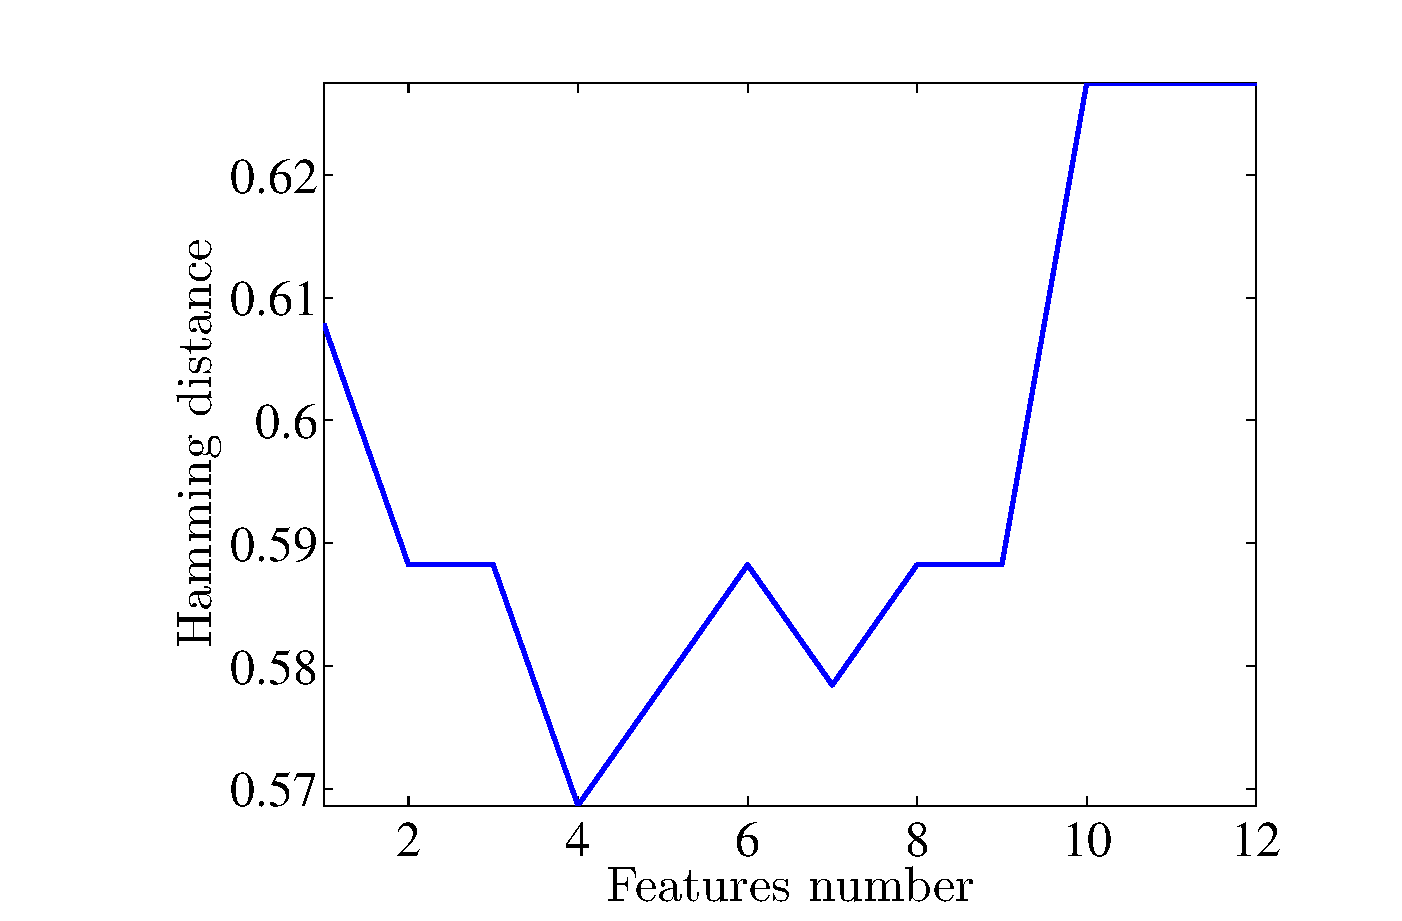
\includegraphics[width=0.5\textwidth]{\hdir/fig1}
\end{figure}
\end{verbatim}
}

Если статья написана по-английски, то это надо указать явно,
сразу после \verb|\begin{document}|
(иначе не~включатся английские переносы слов):
{\small\begin{verbatim}
   \English
\end{verbatim}}

Затем формируется заголовок статьи, включая ссылку на~грант и~аннотацию:
{\small\begin{verbatim}
   \title[Краткое название]{Полное название}
   \author{И.\,О.~Автор, И.\,О.~Соавтор, И.\,О.~Фамилия}
   \email{author@site.ru}
   \organization{Организация, Город}
   \thanks{Ссылка на грант.}
   \abstract{Данная статья посвящена...}
\end{verbatim}}

Также нужно задать второй заголовок
с~переводом названия, фамилий авторов, организации, ссылки на грант и~аннотации на~английский язык:
{\small\begin{verbatim}
   \titleEng[Short title]{Full title}
   \authorEng{F.\,S.~Author, F.\,S.~CoAuthor, and F.\,S.~Name}
   \organizationEng{Organization, City, Country}
   \thanksEng{The paper was supported...}
   \abstractEng{This paper...}
\end{verbatim}}

%Если статья написана по"=английски, то нужно задать второй заголовок
%с~переводом названия, фамилий авторов, организации, ссылки на грант и~аннотации на~русский язык:
%{\small\begin{verbatim}
%   \titleRus[Краткое название]{Полное название}
%   \authorRus{И.\,О.~Автор, И.\,О.~Соавтор, И.\,О.~Фамилия}
%   \organizationRus{Организация, Город}
%   \thanksRus{Работа выполнена при поддержке грантов...}
%   \abstractRus{Данная статья посвящена...}
%\end{verbatim}}

Все эти команды  могут идти в~произвольном порядке и~должны завершаться командой
{\small\begin{verbatim}
   \maketitle
\end{verbatim}}
Данная команда выводит заголовок на основном языке статьи.

Команды \verb|\title| и~\verb|\author| и их аналоги для второго заголовка
могут иметь необязательный аргумент в~квадратных скобках \emph{перед} обязательным "---
это сокращённые версии названия и~списка авторов для колонтитулов.
Если колонтитул умещается в~одну строку, то~соответствующий необязательный аргумент не~нужен.

Кроме того, команды \verb'\author', \verb'\authorRus' могут иметь необязательный аргумент в~квадратных скобках \emph{после} обязательного.
Он~указывается в~тех случаях, когда в~заголовок необходимо вывести дополнительную информацию, например, об организациях:
{\small\begin{verbatim}
   \author{И.\,О.~Автор, И.\,О.~Соавтор}
      [И.\,О.~Автор$^1$, И.\,О.~Соавтор$^2$]
   \organization{$^1$НИИ-X, Москва; $^2$НИИ-Y, Москва}
\end{verbatim}}

Иная расстановка инициалов, пробелов или запятых в~обязательном аргументе команд \verb'\author', \verb'\authorRus' может приводить к~ошибкам в~оглавлении и~авторском указателе.

Ссылка на~грант оформляется как часть заголовка командами \verb'\thanks',  \verb'\thanksRus'
и~выводится в~виде сноски на одной странице с заголовками.

%Аннотация (не~более 10 строк) не~должна содержать ссылок, формул, таблиц, рисунков.

После команды \verb|\maketitle| необходимо включить нумерацию строк, для удобства общения автора с рецензентами.
Для этого за командой \verb|\maketitle| должна следовать команда
{\small\begin{verbatim}
   \linenumbers
\end{verbatim}}

К статье прилагается два списка литературы: к русскоязычной и англоязычной частям.
В русскоязычной статье первым идет список литературы к русскоязычной части.
Далее идет второй заголовок, который выводится командой
{\small\begin{verbatim}
   \maketitleSecondary
   \English
\end{verbatim}}
\noindent
Далее идет список литературы к англоязычной части.

\medskip
Статья должна заканчиваться командой
{\small\begin{verbatim}
   \end{document}
\end{verbatim}}

Каждая статья в~сборнике начинается с~новой страницы,
что позволяет сохранять заданное автором расположение материала на~страницах.
Убедительная просьба: не~использовать команды сокращения вертикальных промежутков
и~другие способы искусственного уплотнения текста.

Текст статьи можно разбивать на~разделы и~параграфы командами
{\small\begin{verbatim}
   \section{Название раздела}
   \paragraph{Название параграфа}
\end{verbatim}}

%Команды \verb'\subsection', \verb'\subparagraph' не~предусмотрены.
В~конце названий разделов и параграфов точка не~ставится.

\section{Списки литературы}

Списки литературы представляются в двух вариантах:
\begin{enumerate}
\item \emph{Литература}~-- к русскоязычной части. Все работы на~языке и алфавите оригинала.
\item \emph{References}~-- к англоязычной части. Русские работы~--  в латинской транслитерации и с~переводом на~английский язык, английские работы и работы на других языках~-- на языке оригинала.
\end{enumerate}

Ссылки на литературу располагаются в каждом из списков литературы в порядке первых упоминаний.
Список литературы \emph{References} приводится полностью отдельным блоком, повторяя все позиции из списка литературы к русскоязычной части, независимо от того, имеются или нет в нем иностранные источники.
Если в списке литературы к русскоязычной части есть ссылки на иностранные публикации, набранные латиницей, они полностью повторяются в списке \emph{References}.
Рекомендуется пользоваться программой автоматического перевода кириллицы в~романский алфавит: \url{http://translit.ru/}, при~этом в~закладке <<варианты...>> следует выбирать опцию BGN.

Список литературы формируется окружением \verb'thebibliography'.
Каждая запись библиографии начинается командой
\verb'\bibitem{'\textit{name}\verb'}'.
Метка \textit{name} позволяет ссылаться на~данную запись командой
\verb'\cite{'\textit{name}\verb'}'.
В~ссылках разрешается указывать несколько меток через запятую без пробелов между метками:
\verb'\cite{'\textit{name$_1$,name$_2$}\verb'}'.
Новая команда \verb'\citenb' даёт ссылку без квадратных скобок, что позволяет делать интервалы;
например,
[\citenb{VoronLatex}--\citenb{Lvovsky}]
было получено так:
\verb'[\citenb{VoronLatex}--\citenb{Lvovsky}]'.
Русские буквы в~именах меток \textit{name} недопустимы.

Названия статей в~сборниках выделяются командой \verb'\BibTitle'.
Если публикация существует только в~электронном виде, веб-ссылка даётся командой \verb'\BibUrl'.
В русскоязычном списке литературы фамилии и~инициалы авторов выделяются командой \verb'\BibAuthor'.

Для повышения точности вычисления показателей цитируемости необходимо по возможности указывать DOI (Digital Object Identifier) публикаций. DOI оформляется с помощью команды \verb'\BibDoi'.
DOI публикации, зарегистрированной в системе Crossref, можно получить по адресу \url{http://www.crossref.org/guestquery/}.

Примеры оформления ссылок на различные виды публикаций:
\begin{itemize}
\item статья из журнала с DOI \cite{article};
\item книга (монография, сборник) \cite{Lvovsky, Kotelnikov, Floudas2009};
\item переводная книга \cite{Goossens}(в списке литературы к~русскоязычной части после названия книги необходимо указать <</ Пер. с англ.>>, а в~конце ссылки указать оригинал книги в~круглых скобках);
\item материалы конференций \cite{inproceedings, inproceedingsEng} (ссылка~\cite{inproceedingsEng} из~англоязычного источника представлена на языке оригинала в обоих списках литературы);
\item технический отчет \cite{techreport};
\item интернет-ресурс \cite{VoronLatex, XYpicUrl, XYpicUrl2, XYpicUrl3, TikZPGFUrl}.
\end{itemize}

\section{Стандартные средства \LaTeX'а}

Нет особых ограничений на~использование основных средств \LaTeX'а~%
\cite{VoronLatex,Goossens,Kotelnikov,Lvovsky}.
В~статью можно вставлять формулы, таблицы, списки, рисунки, сноски, и~т.\,д.
Определения ссылок \verb'\label'
и~команд \verb'\newcommand', \verb'\renewcommand'
действуют только внутри одной статьи;
конфликты с~чужими статьями исключены.

\paragraph{Стандартные пакеты}
Стандартные пакеты подключены в~стилевом файле \verb'jmlda.sty':
\verb'algorithm',
\verb'algorithmic',
\verb'amssymb',
\verb'amsmath',
\verb'array',
\verb'babel',
\verb'balance',
\verb'color',
\verb'cite',
\verb'enumitem',
\verb'euscript',
\verb'graphicx',
\verb'ifthen',
\verb'lineno',
\verb'mathrsfs',
\verb'pb-diagram',
\verb'pgfplots',
\verb'subfig',
\verb'theorem',
\verb'tikz'
\verb'url',
\verb'xy'.
Этими пакетами можно пользоваться, не~вызывая команду \verb'\usepackage'.
Желательно обходиться только этими пакетами.

\paragraph{Формулы}%
Формулы внутри текста, даже очень короткие,
необходимо окружать знаками доллара~\verb'$':

\begin{coderes}
    \verb'число~$-3.14$' & число~$-3.14$ --- верно\\
    \verb'число -3.14'   & число -3.14 --- неверно   \\
    \verb'объект~$x$'    & объект~$x$ --- верно    \\
    \verb'объект x'      & объект x --- неверно
\end{coderes}

Выключные формулы без номера окружаются скобками \verb'\[' и \verb'\]'.
Выключные формулы с~номером окружаются командами
\verb'\begin{equation}' и~\verb'\end{equation}'.
Команда \verb'\label{'\emph{name}\verb'}' между ними
задаёт метку формулы.
Русские буквы в~именах меток~\emph{name} недопустимы.
Метка позволяет ссылаться на~формулу командой
\verb'\eqref{'\emph{name}\verb'}',
например команда \verb'\eqref{eqCases}' даёт~\eqref{eqCases}.

\paragraph{Списки}
Списки оформляются стандартными окружениями \verb|enumerate| или \verb|itemize|.
В~стиле \verb|jmlda.sty| определено окружение \verb|enumerate*|
для списков, в~которых, согласно правилам русской пунктуации:
\begin{enumerate*}
\item номера отделяются скобкой;
\item пункты начинаются со~строчной буквы;
\item и~заканчиваются точкой с~запятой.
\end{enumerate*}
Этот список удобен для перечисления коротких пунктов, умещающихся в~одну строку.
Если пункты длинные, то~лучше воспользоваться стандартным окружением \verb|enumerate|.
В этом случае допустим другой способ оформления списков.

\begin{enumerate}%[label = {(\arabic*)}]
\item Номера отделяются точкой.
\item Пункты начинаются с заглавной буквы.
\item Пункты заканчиваются точкой.
\end{enumerate}

\paragraph{Таблицы}
Таблицы создаются окружением \verb'tabular'
и оформляются как плавающие с~помощью окружения  \verb'table'.
Желательно прижимать их~вверх страницы опцией~\verb|[t]| команды \verb'\begin{table}'.
Подпись делается \emph{над таблицей} командой \verb'\caption', см.~таблицу~\ref{TabExample}.
Команда \verb'\label', определяющая ссылку на~номер таблицы,
обязана идти после \verb'\caption'.
Если таблица не умещается по~ширине колонки,
то~можно уменьшить шрифт до~\verb'\small' или даже \verb'\footnotesize',
либо уменьшить интервалы между колонками:
\verb'\tabcolsep=2pt'.

\begin{table}[t]%\small
    \caption{Подпись размещается над таблицей}
    \label{TabExample}
    \centering\medskip%\tabcolsep=2pt%\small
    \begin{tabular}{lrrr}
    \headline
        Задача
            & \multicolumn{1}{c}{CCEL}
            & \multicolumn{1}{c}{boosting} \\
    \headline
        {\tt Cancer}
            & $\mathbf{3.46}  \pm 0.37$ (3.16)
            & $4.14 \pm 1.48$ \\
        {\tt German}
            & $\mathbf{25.78} \pm 0.65$ (1.74)
            & $29.48 \pm 0.93$ \\
        {\tt Hepatitis}
            & $18.38 \pm 1.43$ (2.87)
            & $19.90 \pm 1.80$ \\
    \hline
    \end{tabular}
\end{table}

\paragraph{Иллюстрации}%
Иллюстрации должны быть подготовлены в~формате \verb'EPS'.
Для преобразования файлов формата \verb'PNG' или \verb'JPEG' в~\verb'EPS' рекомендуется пользоваться утилиту \verb'bmeps', входящую в~пакет MiK\TeX.
Файлы формата \verb'JPEG' могут содержать только иллюстрации, но не графики или диаграммы.
Не~забудьте прислать графические файлы вместе с~\TeX-файлом!

Рисунки вставляются командой \verb|\includegraphics|, желательно с~выравниванием по~ширине колонки: \verb|[width=\linewidth]|.
Если рисунок занимает по~высоте более 1--2~см,
то~он оформляется как плавающая иллюстрация \verb|{figure}| с~прижатием вверх страницы опцией~~\verb|[!ht]|.
Подпись делается \emph{под рисунком} командой \verb|\caption|, см.\,рис.\,\ref{fg:Example}.

Популярные пакеты рисуют графики с подписями, которые трудно читать на бумаге и на слайдах из-за малого размера шрифта. Шрифт на графиках (подписи осей и цифры на осях) должен быть такого же размера, что и основной текст.

\begin{figure}[!ht]
  \subfloat[Первый рисунок]{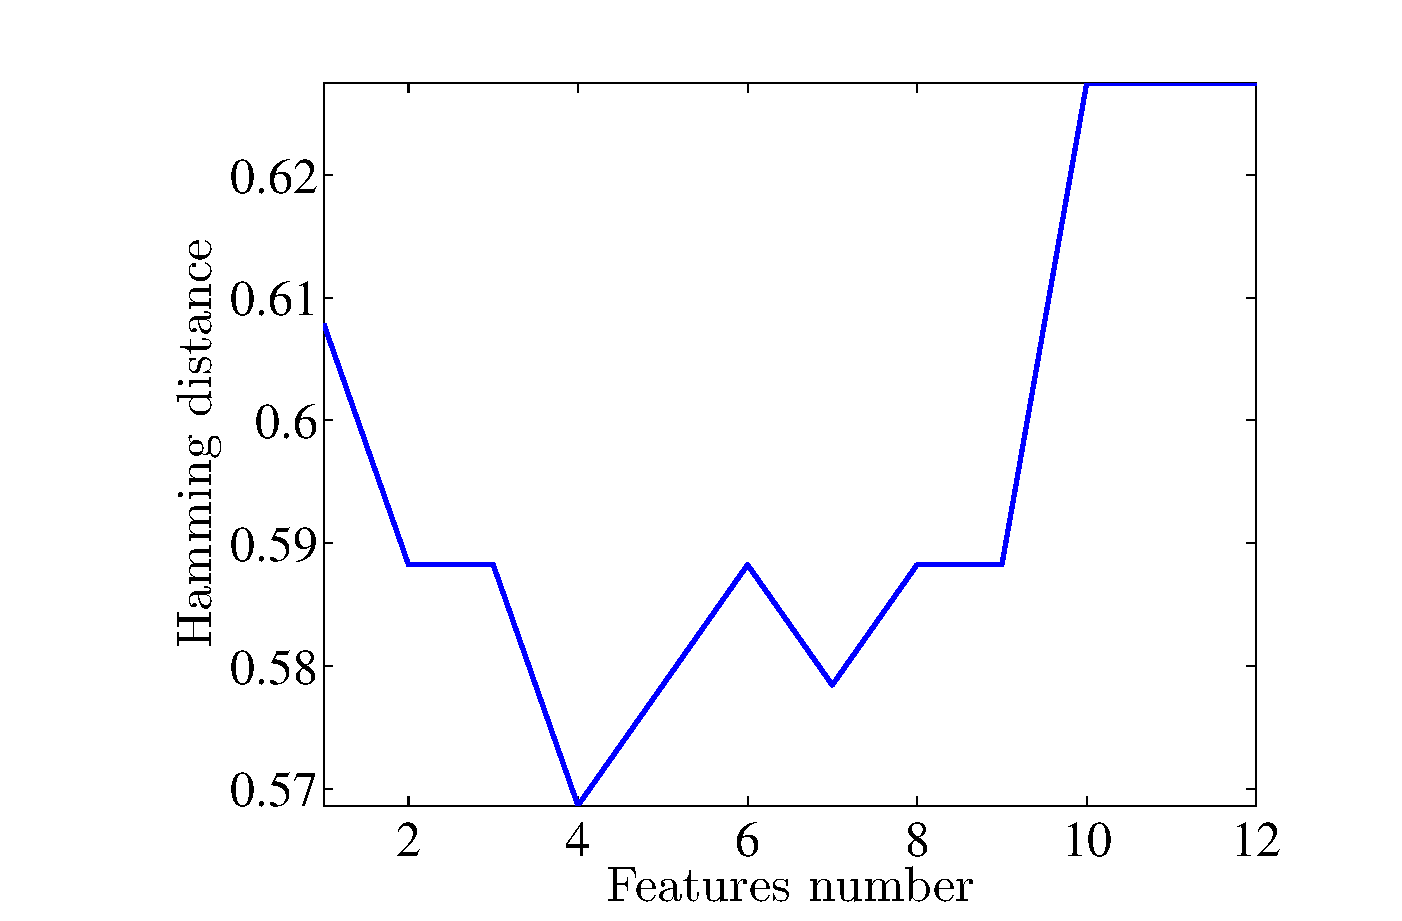
\includegraphics[width=0.5\textwidth]{\hdir/fig1}}
  \subfloat[Второй рисунок]{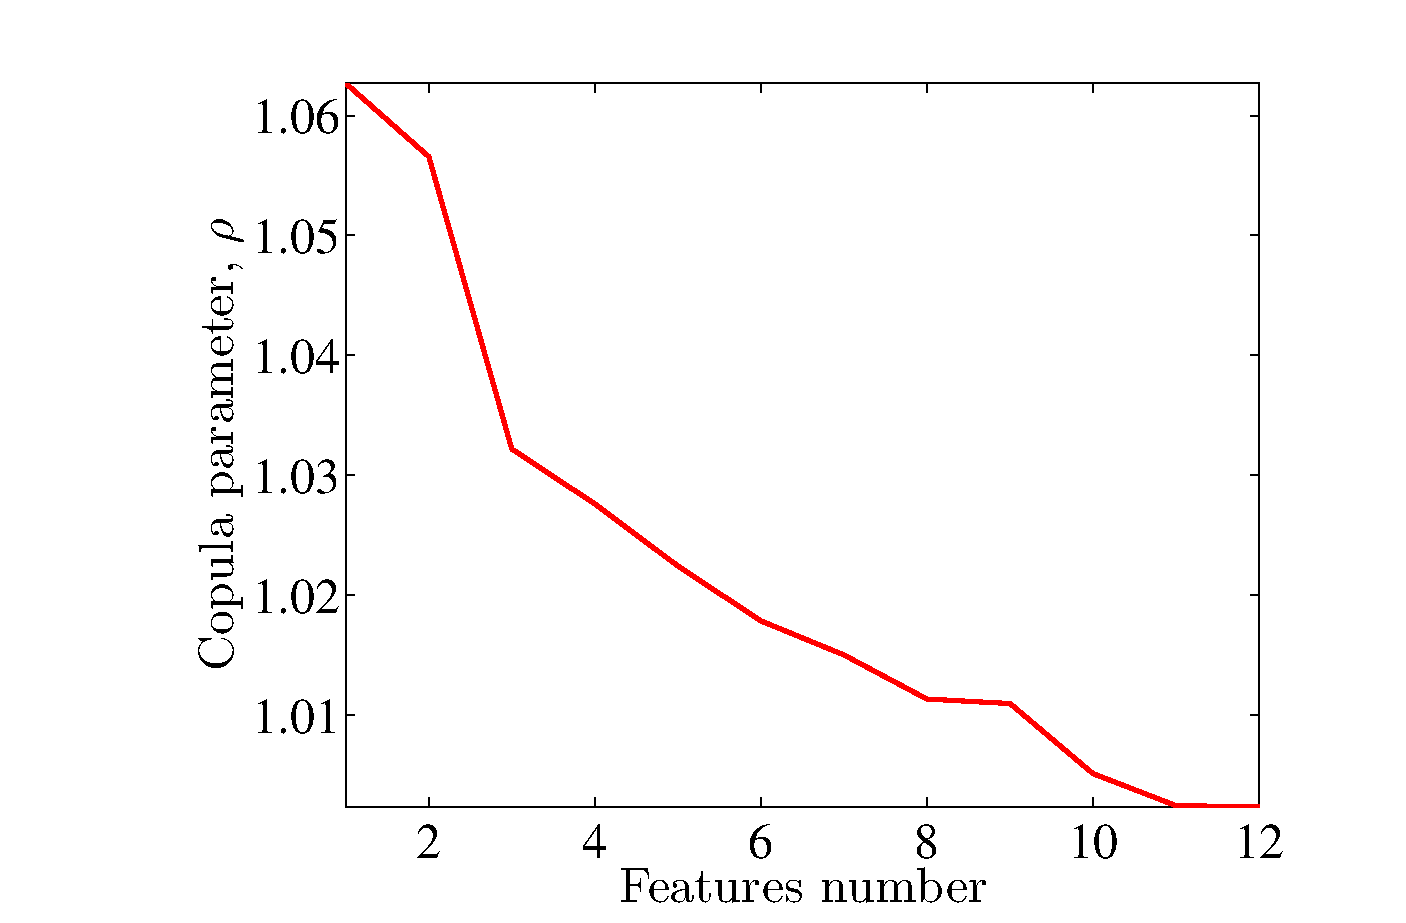
\includegraphics[width=0.5\textwidth]{\hdir/fig2}}
\caption{Подпись размещается под рисунком}
\label{fg:Example}
\end{figure}


При значительном количестве рисунков рекомендуется группировать иx в одном окружении \verb|figure|, как это сделано на рис.~\ref{fg:Example}.
Для этого используется пакет \verb|subfig|.

Определена команда \verb'\XYtext('$x$\verb','$y$\verb'){'\emph{text}\verb'}',
для надписей поверх рисунков.
%TODO
%{До сих пор не решена проблема с~выводом надписи поверх изображения, а~не~под~ним.}
%Например, так сделана надпись <<$Q(\lambda)$>> на~рис.\,\ref{FigExample}.
Координаты левого нижнего угла надписи $(x,y)$ подбираются вручную
относительно правого нижнего угла рисунка.

\paragraph{Оформление иллюстраций}
В популярных пакетах иллюстрации могут быть оформлены следующим образом:
\begin{verbatim}
\begin{figure}[!ht]
  \subfloat[Первый рисунок]
  		{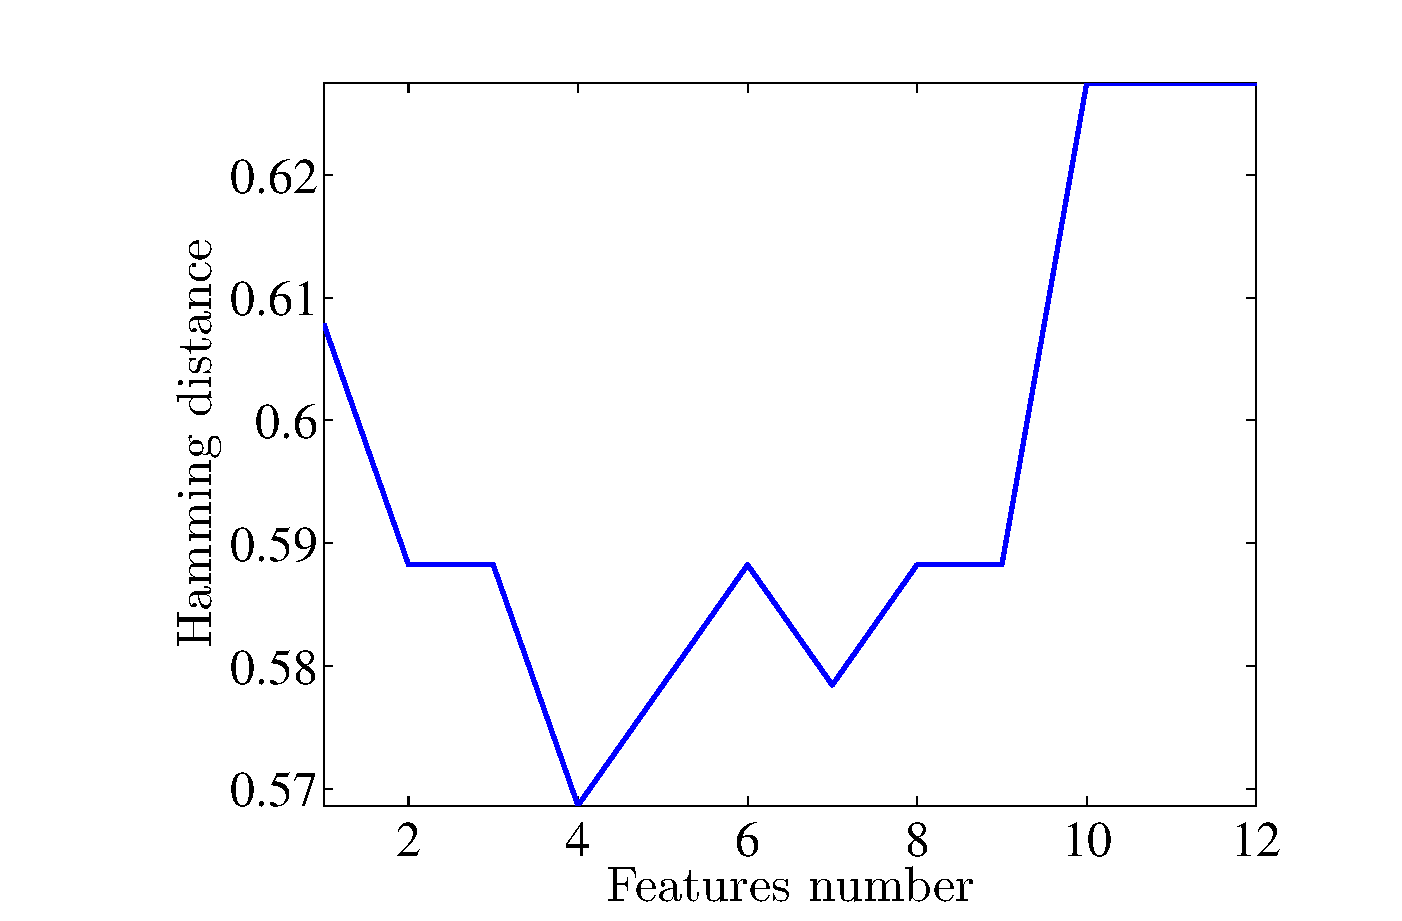
\includegraphics[width=0.5\textwidth]{\hdir/fig1.eps}}
  \subfloat[Второй рисунок]
  	{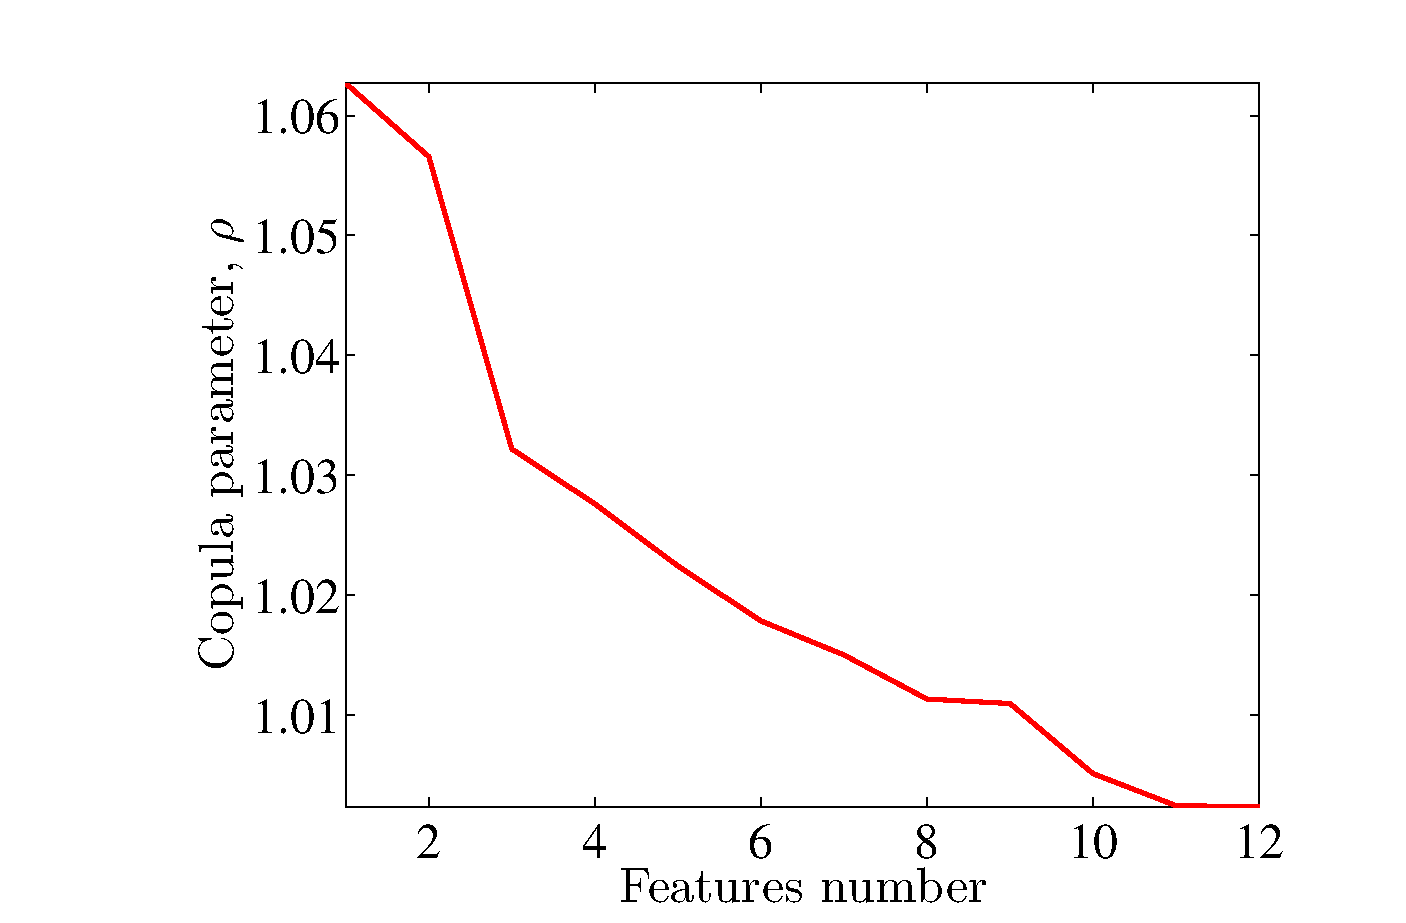
\includegraphics[width=0.5\textwidth]{\hdir/fig2.eps}}
\caption{Подпись размещается под рисунком}
\label{fg:Example}
\end{figure}
\end{verbatim}

\paragraph{Советы по оформлению графиков в системе Matlab}
Приведенный ниже код форматирует рисунок согласно рекомендуемым параметрам:
\begin{itemize}
\item толщина линий равна двум;
\item заголовки осей пишутся с большой буквы;
\item необходимо включить интерпретатор \LaTeX\ для корректного отображения формул на осях;
\item заголовок графика отсутствует (чтобы не дублировать подпись графика в статье).
\end{itemize}

\begin{verbatim}
h = figure; hold('on');
plot(xi,y,'r-', 'Linewidth', 2);
plot(xi,y,'b.', 'MarkerSize', 12);
axis('tight');
xlabel('Time, $\xi$', 'FontSize', 24, 'FontName', ...
       'Times', 'Interpreter','latex');
ylabel('Value, $y$', 'FontSize', 24, 'FontName', ...
       'Times', 'Interpreter','latex');
set(gca, 'FontSize', 18, 'FontName', 'Times')
saveas(h,'ModelOne.eps', 'psc2'); % save to EPS
\end{verbatim}
Рекомендуется сразу сохранять файлы в формате \verb'EPS'.
На рис.~\ref{fg:ExampleMatlab} дан пример графика, удовлетворяющего описанным выше требованиям.

\begin{figure}[!th]
	\begin{center}
 		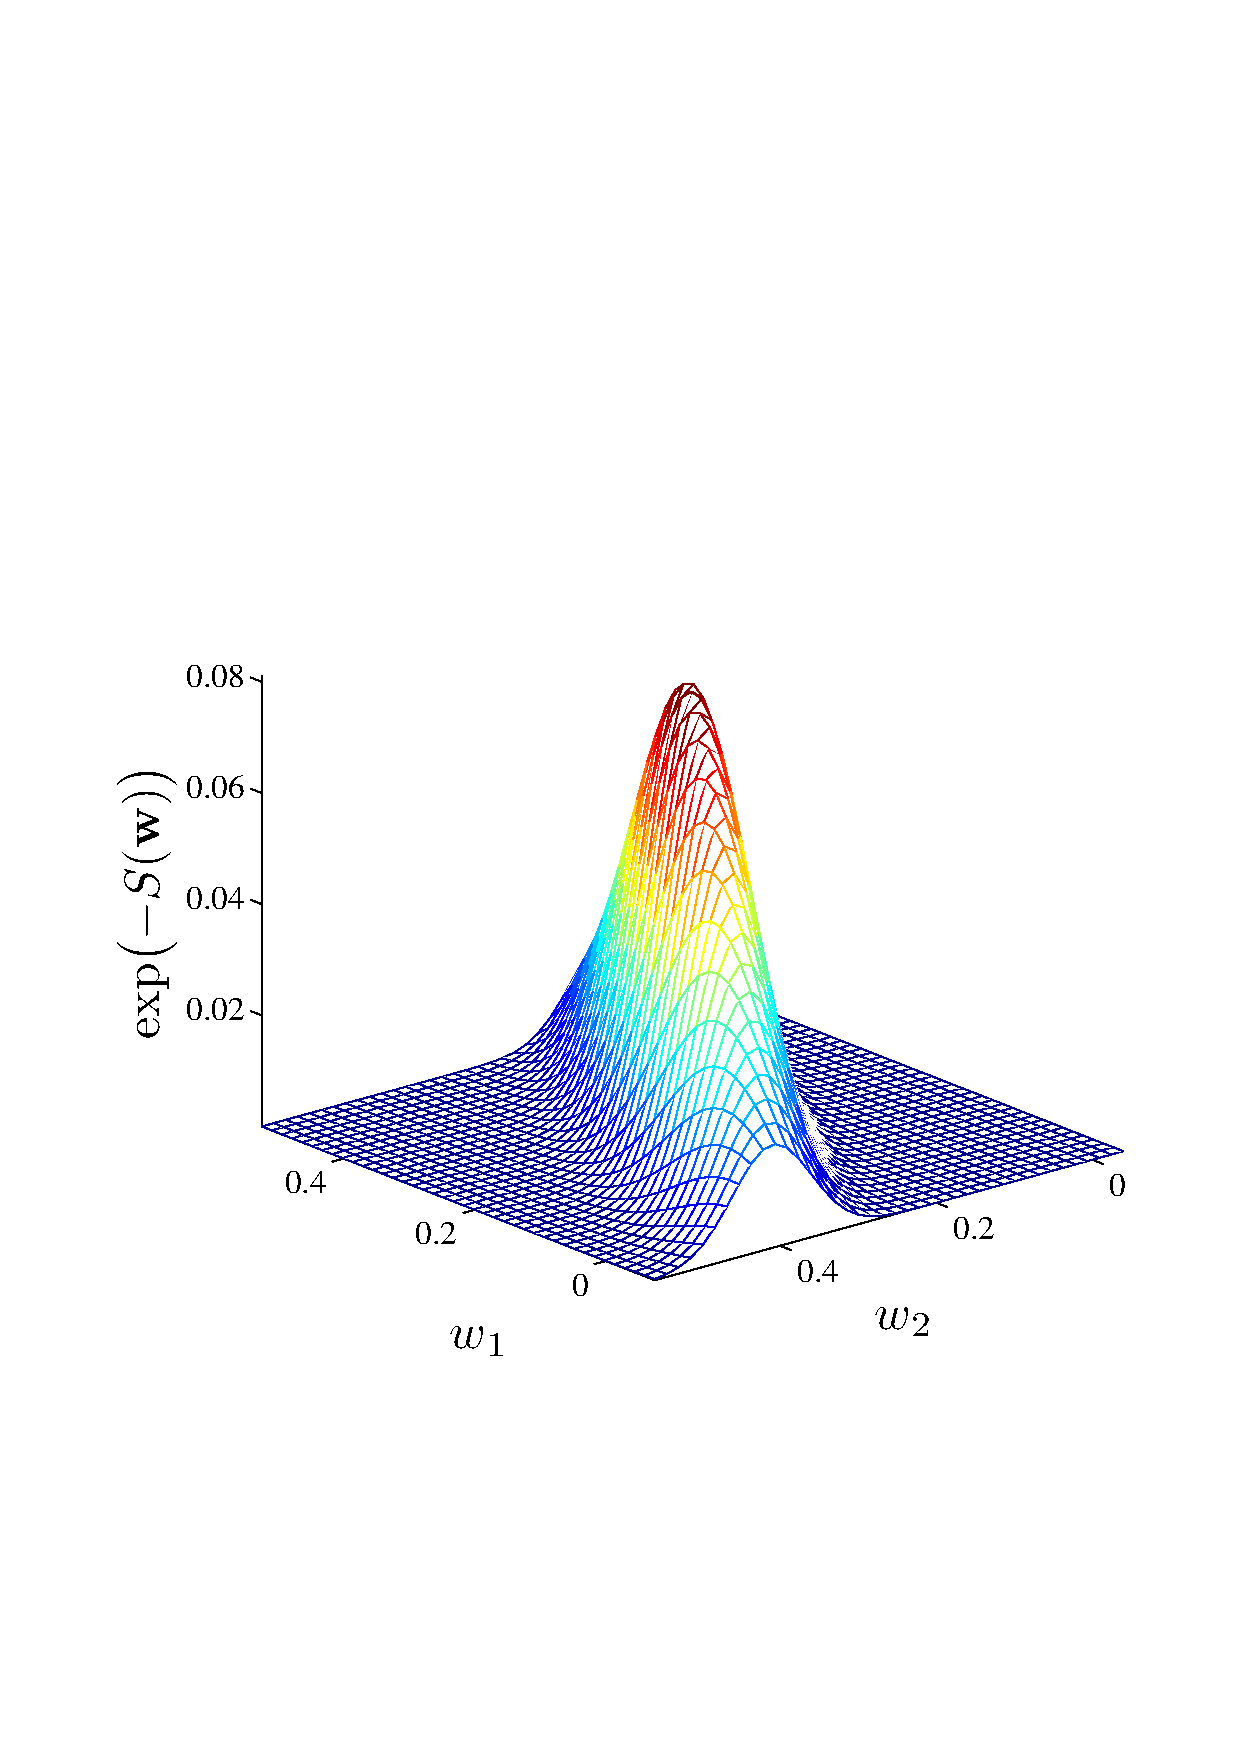
\includegraphics[width=0.5\textwidth]{\hdir/fig5}	
	\end{center}
\caption{Пример графика, подготовленного в системе Matlab}
\label{fg:ExampleMatlab}
\end{figure}


\paragraph{Верстка диаграмм}
Xy-pic~--- пакет \LaTeX, специализированный под создание диаграмм.
Руководство по использованию пакета дано в~\cite{XYpicUrl, XYpicUrl2, XYpicUrl3}.
			
Простой пример использования пакета Xy-pic вместе с кодом его реализации:
\begin{displaymath}
    \xymatrix{
        A \ar[r]^f \ar[d]_g & B \ar[d]^{g'} \\
        D \ar[r]_{f'}       & C }
\end{displaymath}
\begin{verbatim}
	\begin{displaymath}
    \xymatrix{
        A \ar[r]^f \ar[d]_g & B \ar[d]^{g'} \\
        D \ar[r]_{f'}       & C }
	\end{displaymath}
\end{verbatim}

Пример более сложной диаграммы:
\[
\begin{centering}
\xymatrix{
\Phi_1\ar[d]|-{n_1}&\Psi_1\ar[l]_{r_1}\ar[r]^{l_1}\ar[d]|-{k_1}&\Lambda_1\ar[dr]|-{m_1}\ar@/^1pc/@{-->}[drrr]|-(.75){i}&   &\Lambda_2\ar[dl]|-{m_2}\ar@/_1pc/@{-->}[dlll]|-(.75){j}&\Psi_2\ar[l]_{l_2}\ar[r]^{r_2}\ar[d]|-{k_2}&\Phi_2\ar[d]|-{n_2}\\
\Omega_1&\Delta_1\ar[l]_{g_1}\ar[rr]^{f_1}&   &\Gamma  &   &\Delta_2\ar[ll]_{f_2}\ar[r]^{g_2}&\Omega_2
}
\end{centering}
\]
Больший спектр возможностей для~подготовки векторной графики и построения диаграмм предоставляют пакеты TikZ и PGF~\cite{TikZPGFUrl}.

\paragraph{Оформление графиков в Inkscape}
Пример использования векторного графического редактора Inkscape, удобного для создания технических иллюстраций:
\begin{enumerate}
\item Нарисовать изображение, используя, где необходимо, формулы в формате \LaTeX.
\item Сохранить изображение в формате \verb'EPS', используя дополнительную опцию <<создать файл latex>>. На выходе сгенерируется два файла --- \verb|image.eps| и    \verb|image.eps_tex|, второй можно редактировать в \TeX-редакторе.
\item Вставить файл \verb|image.eps_tex| в код статьи, заменив при этом
\begin{verbatim}
\includegraphics[width=<desired width>]{\hdir/image.eps}
\end{verbatim}
на
\begin{verbatim}
\def\svgwidth{<desired width>}
\input{\hdir/image.eps_tex}
\end{verbatim}
\end{enumerate}

Пример использования редактора показан на рис.~\ref{fg:ExampleInk}. Слева показано исходное изображение в редакторе InkScape. Справа~--- полученное после компиляции в системе \LaTeX\ изображение в формате \verb'EPS'.

\begin{figure}[!ht]
  \subfloat[Исходный рисунок в редакторе Inkscape]{
  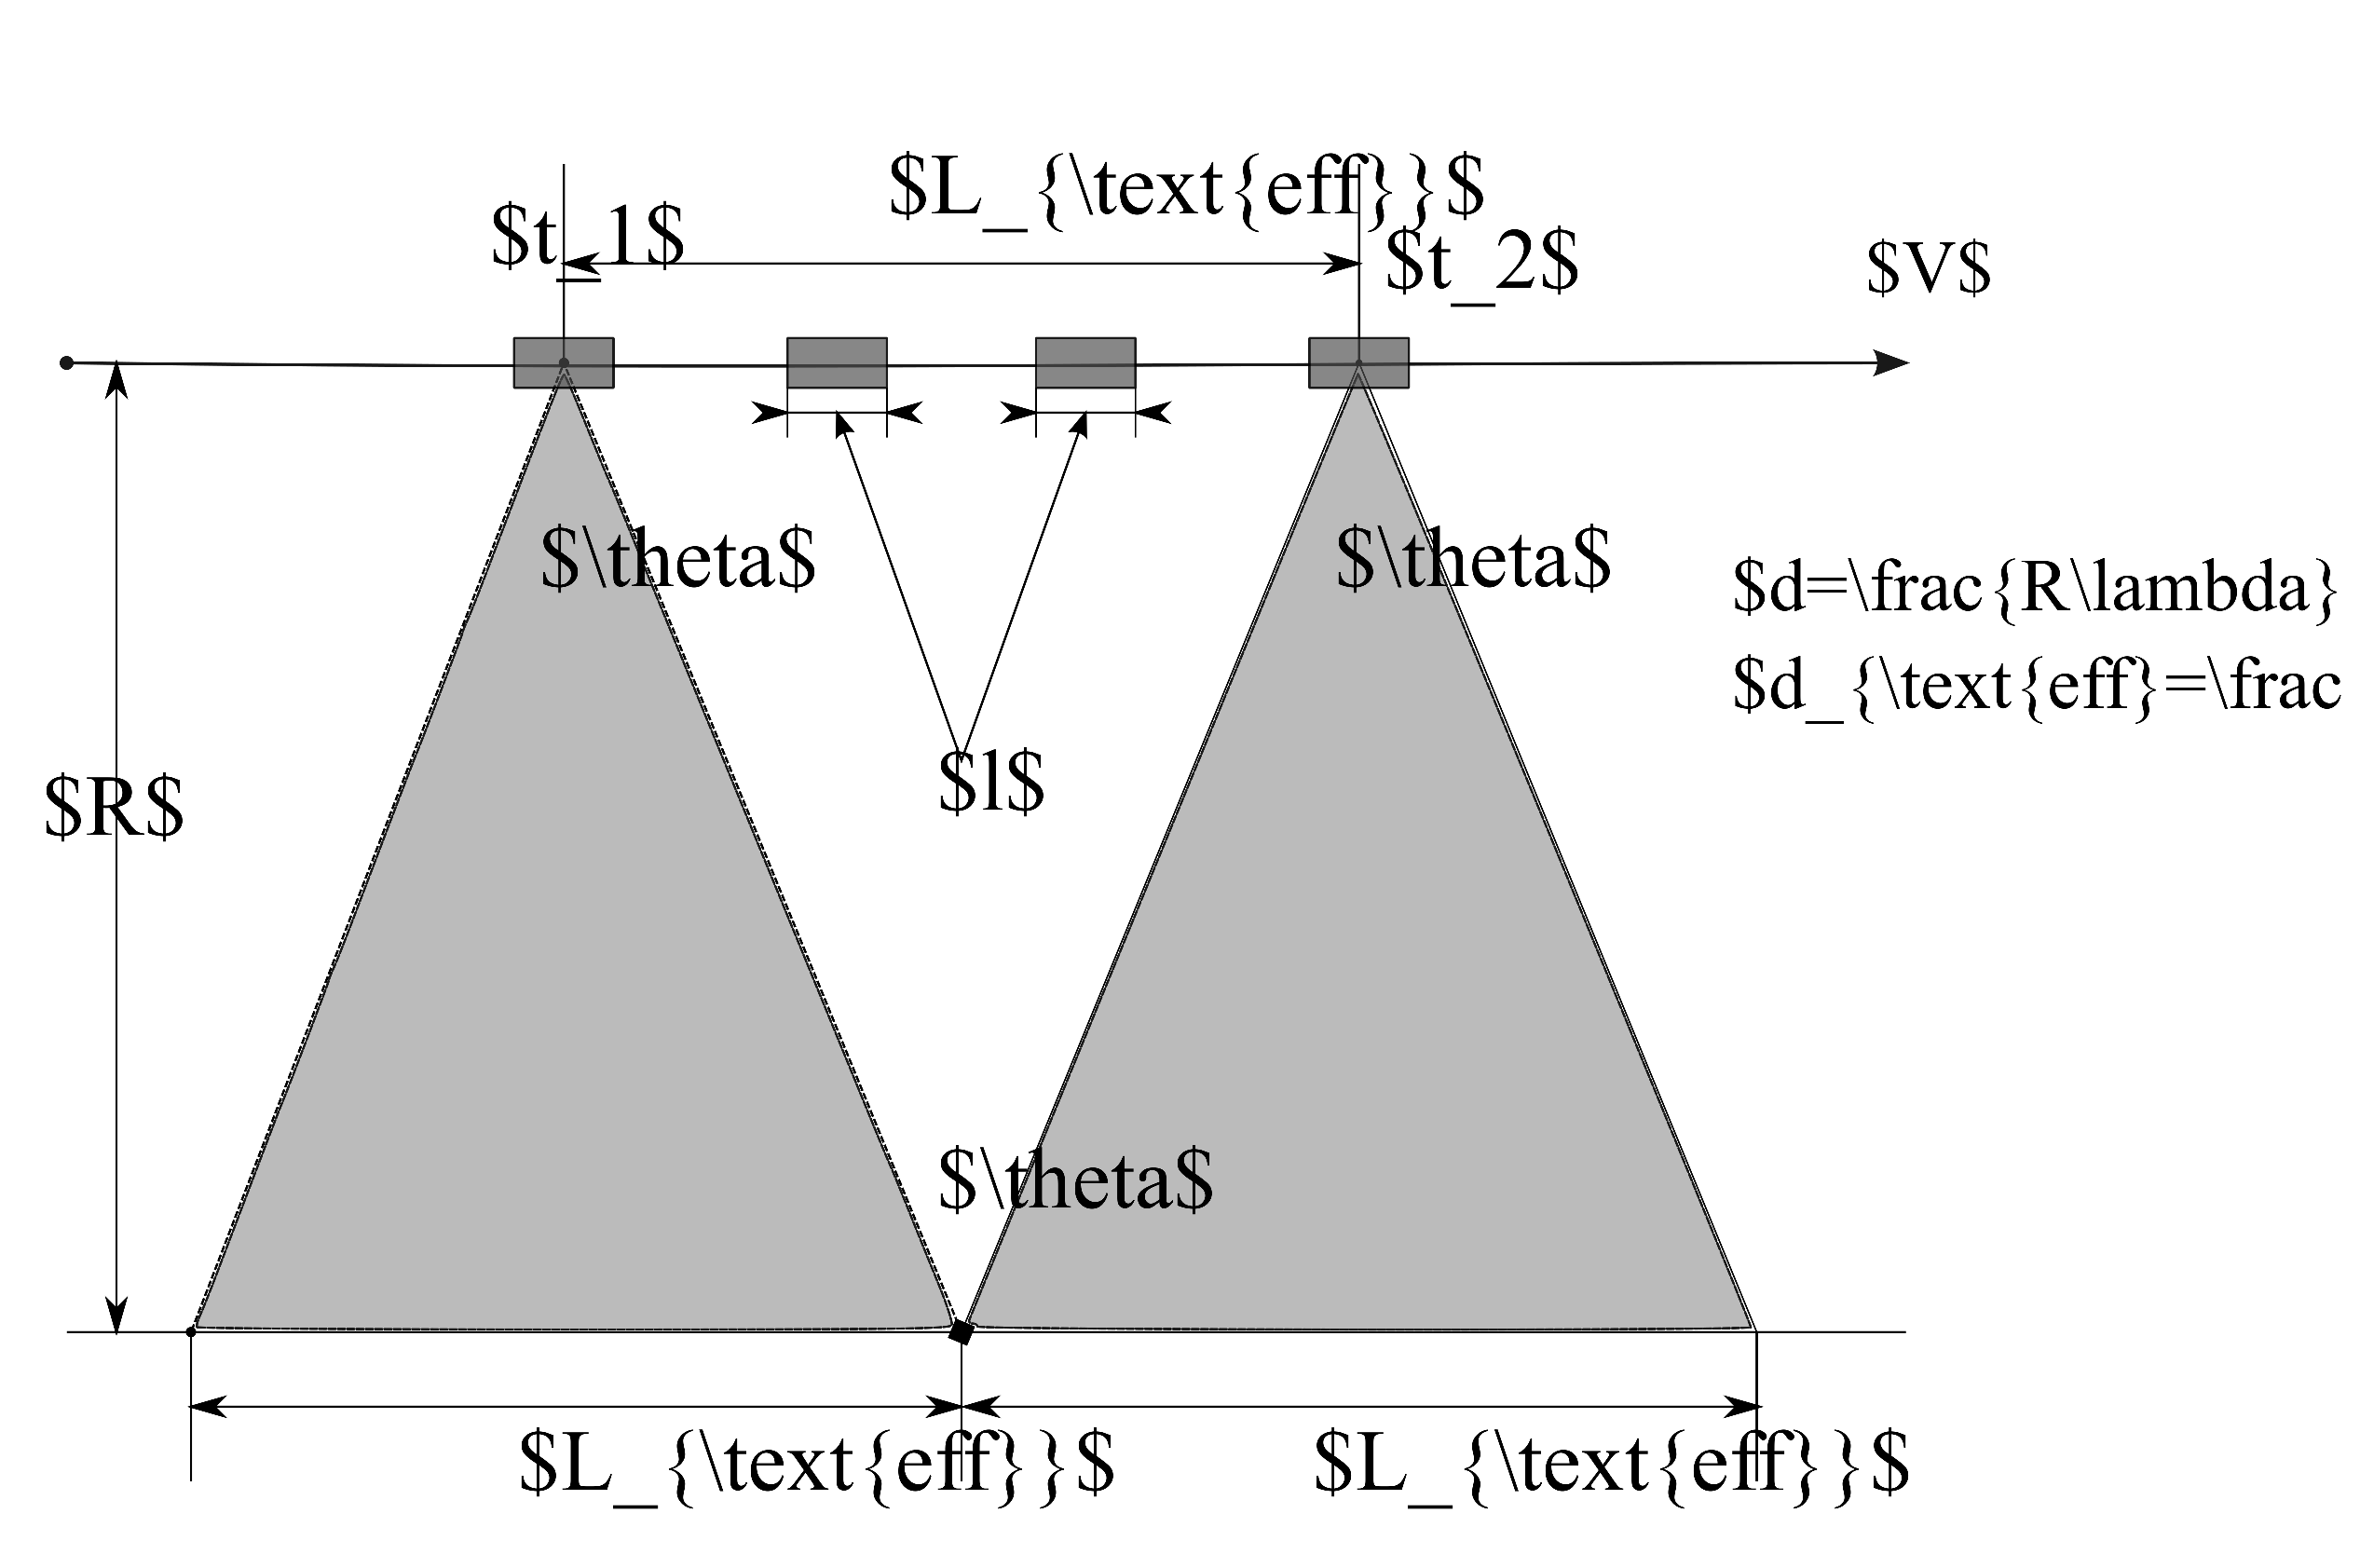
\includegraphics[width=0.5\textwidth]{\hdir/fig3}
  }
  \subfloat[Полученный рисунок]{
   \def\svgwidth{0.5\textwidth}
  \input{\hdir/fig4.eps_tex}
  }\\
\caption{Пример использования редактора InkScape}
\label{fg:ExampleInk}
\end{figure}

\paragraph{Сноски}
Сноски делаются командой \verb'\footnote{'\emph{text}\verb'}'%
\footnote{Текст сноски указывается в~аргументе \emph{text}.}.
Желательно избегать использования сносок в научной статье.

\paragraph{Глобальные ссылки}
В~стиле \verb'jmlda.sty' определены команды
\verb'\globallabel',
\verb'\globalref',
\verb'\globalpageref',
позволяющие сослаться из~одной статьи на~любое место в~другой статье.
Это полные аналоги стандартных команд
\verb'\label',
\verb'\ref',
\verb'\pageref',
но~определяемые ими метки доступны во~всём сборнике.
Типичное применение этой возможности "---
указать в~библиографии диапазон страниц другой статьи <<в~настоящем сборнике>>:
{\small\begin{verbatim}
   C.\,\globalpageref{Kozlov:begin}--%
       \globalpageref{Kozlov:end}
\end{verbatim}}
Для каждой статьи в~сборнике по умолчанию определены две метки\\
{\verb'\globallabel{'\textit{file}\verb':begin}' и~\verb'\globallabel{'\textit{file}\verb':end}'},
где \textit{file} "--- имя \TeX-файла статьи, без указания расширения.

\paragraph{Ссылки на сайты}
Ссылки на сайты делаются командой \verb'\url'.
При вёрстке документа в~формате \verb'PDF' ссылки становятся активными,
хотя не~подчёркиваются и~не выделяются цветом.
Пример:~\verb'\url{www.jmlda.org}'.

\section{Математические обозначения}

Следование приводимым ниже рекомендациям
способствует большему единообразию в~обозначениях
и~облегчает подготовку сборника.

Целочисленные интервалы обозначаются только как $1,\dots,n$.
Варианты $\overline{1,n}$ или $1,\dots,i,\dots,n$ или $1,2,\dots,n$
недопустимы.
То~же относится к~векторам и~спискам переменных вида $x_1,\dots,x_n$.

В~качестве десятичного разделителя используется запятая:
в~формуле \verb|$3{,}14$|, в~тексте \verb|3,14|.

Числовые множества $\NN$, $\ZZ$, $\RR$, $\CC$
делаются командами \verb'\NN', \verb'\ZZ', \verb'\RR', \verb'\CC'.

В~стиле \verb'jmlda.sty' переопределены команды
\verb$\geq$,
\verb$\leq$,
\verb$\emptyset$,
\verb$\epsilon$,
\verb$\kappa$,
\verb$\phi$
математических символов
$\geq$,
$\leq$,
$\emptyset$,
$\epsilon$,
$\kappa$,
$\phi$.

Математические операторы $\lim$, $\inf$, $\sup$, $\min$, $\max$
переопределены так, что пределы всегда ставятся снизу, а~не~сбоку.

Определены математические операторы:
$\argmin$,
$\argmax$,
$\diag$,
$\sign$,
$\Tr$,
$\const$
командами
\verb$\argmin$,
\verb$\argmax$,
\verb$\diag$,
\verb$\sign$,
\verb$\Tr$,
\verb$\const$.

Команды \verb'\myop' и~\verb'\mylim' производят
новые операторы, не~предусмотренные \LaTeX'ом:

\begin{coderes}
    \verb'$\myop{Ker} f$'            & $\myop{Ker} f$ \\
    \verb'$A_{\myop{Ker} f}$'        & $A_{\myop{Ker} f}$ \\
    \verb'$\myop{Hom}_\Phi(A,B)$'    & $\myop{Hom}_\Phi(A,B)$ \\
    \verb'$\mylim{Hom}_\Phi(A,B)$  ' & $\mylim{Hom}_\Phi(A,B)$
\end{coderes}

Для выделения векторных и~матричных величин прямым жирным шрифтом
предусмотрена команда \verb'\vec{'\textit{формула}\verb'}'.

\paragraph{Линейная алгебра}
\begin{coderes}
    \verb'$\rank A$'                 & $\rank A$ \\
    \verb'$\Tr A$'                   & $\Tr A$ \\
    \verb'$\diag (d_1,\dots,d_n)$'   & $\diag (d_1,\dots,d_n)$ \\
    \verb'$A\T$'                     & $A\T$ \\
    \verb'$u\T F\T F u$'             & $u\T F\T F u$ \\
    \verb'$\vec x$'                  & $\vec x$ \\
    \verb'$\Omega \neq \vec\Omega$'  & $\Omega \neq \vec\Omega$ \\
    \verb'$e^{-\vec{x\T\Sigma x}}$ ' & $e^{-\vec{x\T\Sigma x}}$ (верно)\\
    \verb'$e^{-x\T\Sigma x}$'        & $e^{-x\T\Sigma x}$ (неверно)
\end{coderes}

\paragraph{Теория вероятностей}
\begin{coderes}
    \verb'$\Prob\{x\colon x\in A\}$' & $\Prob\{x\colon x\in A\}$ \\
    \verb'$\Expect \xi$'             & $\Expect \xi$ \\
    \verb'$\Var \xi$'                & $\Var \xi$ \\
    \verb'$\Normal(\mu,\Sigma)$'     & $\Normal(\mu,\Sigma)$ \\
    \verb'$p(x\cond y)$'             & $p(x\cond y)$
\end{coderes}

В~условных вероятностях команда \verb'\cond'
даёт правильные пробелы вокруг вертикальной черты.

\paragraph{Теория вычислительной сложности}
\begin{coderes}
    \verb'$\P$                     ' & $\P$ \\
    \verb'$\NP$'      & $\NP$ \\
    \verb'$\DTIME$'   & $\DTIME$ \\
    \verb'$\MaxSNP$'  & $\MaxSNP$ \\
    \verb'$\Apx$'     & $\Apx$ \\
    \verb'$\PC$'      & $\PC$ \\
    \verb'$\MinPC$'   & $\MinPC$ \\
    \verb'$\threeSAT$'& $\threeSAT$ \\
    \verb'$\GapSAT$'  & $\GapSAT$
\end{coderes}\\
Легко определять собственные такие команды для новых классов сложности и~задач,
например, класс~\NP\ и задача \MinPC\ были определены так:
{\small\begin{verbatim}
   \def\NP{\CCfont{NP}}
   \def\MinPC{\CPfont{MinPC}}
\end{verbatim}}

Все эти команды могут употребляться как внутри формул, так и~непосредственно в~тексте.

Для оформления условных конструкций пользуйтесь стандартным окружением \verb'cases'.
Текст внутри формул выводится командой \verb'\text':
\begin{equation}\label{eqCases}
    y(x,\alpha) = \begin{cases}
        -1, & \text{если } f(x,\alpha)<0;  \\
        +1, & \text{если } f(x,\alpha)\geq 0.
    \end{cases}
\end{equation}
{\small\begin{verbatim}
   \begin{equation}\label{eqCases}
      y(x,\alpha) = \begin{cases}
         -1, & \text{если } f(x,\alpha)<0; \\
         +1, & \text{если } f(x,\alpha)\geq 0.
      \end{cases}
   \end{equation}
\end{verbatim}}

Чтобы размер скобок соответствовал размеру обрамляемой формулы,
пользуйтесь командами \verb'\left' и~\verb'\right'.
Однако в~простых случаях эти команды не~нужны и~только загромождают текст.
Лучше записать \verb'f(x_i)', чем \verb'f\left(x_i\right)'
"--- результат в~обоих случаях будет одинаков.

Для вставки матрицы в~строку текста
$
    \bigl(
    \begin{smallmatrix}
        a & b & c \\
        1 & 2 & 3
    \end{smallmatrix}
    \bigr)
$
используйте окружение \verb'smallmatrix'.
Все остальные способы дают некрасивый результат.

\paragraph{Окружения типа теорем}
Следующие окружения выводят заключённый в~них текст {\slshape наклонным шрифтом}:
\verb'Def' или \verb'Definition' "--- Определение,
\verb'Theorem' "--- Теорема,
\verb'Lemma' "--- Лемма,
\verb'State' "--- Утверждение,
\verb'Corollary' "--- Следствие.

Следующие окружения выводят заключённый в~них текст обычным шрифтом:
\verb'Axiom' "--- Аксиома,
\verb'Problem' "--- Задача,
\verb'Example' "--- Пример,
\verb'Remark'~--- \mbox{Замечание,}
\verb'Hypothesis' "--- Гипотеза.


\section{Рекомендации по оформлению}

Придерживаясь следующих правил, авторы существенно облегчают подготовку сборника.
%Общие трудозатраты на~подготовку сборника существенно снижаются,
%если авторы придерживаются нескольких несложных правил, приведённых ниже.
%Авторам будет также полезно ознакомиться с~типичными ошибками,
%приведёнными в~рекомендациях корректорам и~рецензентам.

%По~возможности старайтесь вставлять рисунки и~таблицы как плавающие вверху страницы,
%и~только при острой необходимости вставляйте по~месту первого упоминания в~тексте.

\paragraph{Некоторые правила типографики}
Скобки всех видов набираются вплотную к тексту, который они окружают.
Знаки препинания набираются
слитно с~предшествующим текстом и~отдельно от~последующего.

Кавычки делаются в~русском тексте так: \verb'<<'\emph{текст}\verb'>>',
в~английском так: \verb|``|\emph{text}\verb|''|.
Использовать символ \verb'"' нельзя!

Многоточия в~тексте и~формулах делаются командой \verb'\dots'.

Тире отделяется от~предшествующего текста неразрывным пробелом:
\verb*'Знание~--- сила'.

В~длинных словах с~дефисом, таких, как <<счётно"=аддитивно>>,
дефис делается командой \verb'"=', иначе слово не~будет переноситься:
\verb'счётно"=аддитивно'.
Команда \verb'"~' запрещает перенос по~дефису:
$F$"~пре\-образование,
\verb'$F$"~пре\-образование'.
%В~английских текстах команды \verb'"=' и~\verb'"~' не~работают.

Неразрывный пробел~\verb'~' ставится
между коротким предлогом и~последующим словом,
\mbox{а~также} между очень короткой формулой и~связанным с~ней по~смыслу словом:
\verb'число~$N$ в~$k$~раз' \verb'больше, чем~$n$'.

Между идущими подряд формулами иногда нужен дополнительный пробел:
\begin{coderes}
    \verb'$a=1$, $b=2$'       & $a=1$, $b=2$ ~~~--- плохо \\
    \verb'$a=1$,\: $b=2$'  & $a=1$,\: $b=2$  ~~~--- хорошо \\
    \verb'$a=1$,\quad $b=2$'  & $a=1$,\quad $b=2$ ~~~--- хорошо
\end{coderes}

Иногда в~формуле надо убрать пробелы вокруг знака операции.
Например, если {знак~$\times$}\\ используется не~как произведение,
а~для указания размеров матрицы или растрового изображения,
то~его лучше не~окружать пробелами:

\begin{coderes}
    \verb'$640\times 480$'  & $640\times 480$ ~~~--- плохо \\
    \verb'$640{\times}480$' & $640{\times}480$ ~~~--- хорошо
\end{coderes}

Дополнительный пробел \verb'\quad' рекомендуется вставлять
между длинными выражениями, идущими через запятую в~выключной формуле.

Короткий пробел \verb'\,' ставится
после знака номера: \verb|\No\,6|;
в~инициалах: \verb|И.\,В.\,Анов|;
в~сокращениях: \verb|т.\,к.|; \verb|т.\,е.|; \verb|и~т.\,д.|

Не~следует использовать жирный шрифт для выделения
\emph{важных слов} или \emph{терминов}.
Это делается командой \verb'\emph{'\emph{текст}\verb'}'.

\paragraph{Правила форматирования}
Форматирование исходного кода облегчает его чтение и~работу над корректурой:
\begin{itemize}
\item
    начинайте каждое предложение с~новой строки;
\item
    набирайте отдельной строкой команды
    \verb'\begin', \verb'\end', \verb'$$', \verb'\[', \verb'\]',
    \verb'\section', \verb'\subsection', \verb'\paragraph',
    \verb'\item', \verb'\bibitem', \verb'\par', \verb'\label';
\item
    внутритекстовые формулы, за~исключением совсем коротких,
    набирайте отдельной строкой;
\item
    длинные описания формул разбивайте на строки;
    используйте табуляции для выделения вложенных скобок и~логически обособленных частей формул,
    как показано в~Примере~\ref{exExample}.
\end{itemize}

\begin{Example}
\label{exExample}
    Форматирование сложной формулы:
    \begin{align*}
    R'_N(F)
        = \frac1N \sum_{i=1}^N
        \Bigl(
            & P(+1\cond x_i) C\bigl(+1,F(x_i)\bigr)
        +{} \\ {}+{}
            & P(-1\cond x_i) C\bigl(-1,F(x_i)\bigr)
        \Bigr).
    \end{align*}
\end{Example}
{\small\begin{verbatim}
    \begin{align*}
       R'_N(F)
       = \frac1N \sum_{i=1}^N
        \Bigl(
          & P(+1\cond x_i) C\bigl(+1,F(x_i)\bigr)
        +{} \\ {}+{}
          & P(-1\cond x_i) C\bigl(-1,F(x_i)\bigr)
        \Bigr).
    \end{align*}
\end{verbatim}}

\paragraph{Правила оформления \emph{References}}
\begin{itemize}
\item вместо переводного издания книги (монографии) необходимо представлять описание ее оригинальной версии; переводная версия может быть также описана как дополнительные сведения в скобках;
\item перевод заглавия статьи или источника берется в~квадратные скобки;
\item если известно переводное название статьи в~том виде, как оно указано в~журнале, то транслитерация заглавия не требуется, но в~скобках после описания указывается язык публикации (In Russian);
\item если нужно сократить описание, то лучше приводить переводное описание с~указанием в скобках (In Russian);
%\item если описываемая публикация имеет doi (digital object identifier), его обязательно надо указывать в описании;
\item для неопубликованных документов можно делать самое короткое название с указанием в скобках (unpubl.);
\item для сокращения названий источников желательно использовать аббревиатуры журналов в соответствиями с рекомендациями Web of Science (см., например, \url{http://images.webofknowledge.com/WOK46/help/WOS/A_abrvjt.html});
\item все основные выходные издательские сведения должны быть представлены на английском языке; в описаниях журналов это обозначение тома, номера, страниц; в описаниях книг~-- место издания и обозначение издательства, за исключением собственного непереводного имени издательства, которое транслитерируется.
\end{itemize}

\paragraph{Формирование списка литературы с помощью Bib\TeX}

Если список литературы к русскоязычной части оформлен в файле \\ \verb'Author2017Keyword_rus.bib', то для~формирования списка литературы в~автоматизированном режиме необходимо
\begin{enumerate*}
\label{en:1}
\item добавить \verb'\bibliographystyle{jmlda-rus}' перед \verb'\begin{document}'
\item в конце текста статьи перед \verb'\end{document}' необходимо добавить
{\small\begin{verbatim}
  \bibliography{Author2017Keyword_rus}
\end{verbatim}}
\item скомпилировать статью следующей последовательностью команд:
{\small\begin{verbatim}
	latex Author2017Keyword
	bibtex Author2017Keyword
\end{verbatim}}
\label{en:3}
\end{enumerate*}

После успешной компиляции в файле \verb'Author2017Keyword.bbl' содержится список литературы к русскоязычной части.
Если списка литературы к англоязычной части нет, то далее необходимо скопировать содержимое этого файла в текст статьи и скомпилировать.
Если же список литературы \emph{References} находится в~\verb'Author2017Keyword_eng.bib', то необходимо \verb'Author2017Keyword.bbl' переименовать на \verb'Author2017Keyword_rus.bbl' и повторить действия~\ref{en:1})---\,\ref{en:3}), заменив \verb'Author2017Keyword_rus' и \verb'jmlda-rus' на~\verb'Author2017Keyword_eng' и \verb'jmlda-eng'.
Затем вставить содержимое обоих файлов \verb'Author2017Keyword_rus.bbl' и \\ \verb'Author2017Keyword.bbl' в исходный текст статьи и скомпилировать.

\begin{thebibliography}{99}
\bibitem{VoronLatex}
    \BibAuthor{Воронцов~К.\,В.}
    \BibTitle{\LaTeXe\ в~примерах}. 2006.
    URL: \BibUrl{http://www.ccas.ru/voron/download/voron05latex.pdf}.

\bibitem{Goossens}
    \BibAuthor{Гуссенс~М., Миттельбах~Ф., Cамарин~А.}
    \BibTitle{Путеводитель по пакету \LaTeX\ и~его расширению \LaTeXe} / Пер. с англ.~---
    М.:~Мир, 1999. 606~с.
    (\BibAuthor{Goossens M., Mittelbach F., Samarin A.}
     \BibTitle{The \LaTeX\ companion}.~---
     2nd ed.~--- Reading, MA, USA: Addison-Wesley, 1994. 528 p.)

\bibitem{Kotelnikov}
    \BibAuthor{Котельников~И.\,А., Чеботаев~П.\,З.}
    \BibTitle{\LaTeXe\ по-русски.}~---
    Hовосибирск:~Cибирский хронограф, 2004. 489~с.

\bibitem{Lvovsky}
    \BibAuthor{Львовский~С.\,М.}
    \BibTitle{Набор и вёрстка в пакете~\LaTeX}.~---
    3-е изд.~---
    М.:~МЦHМО, 2003. 448~с.

\bibitem{article}
    \BibAuthor{Загуренко~А.\,Г., Коротовских~В.\,А., Колесников~А.\,А., Тимонов~А.\,В., Кардымов~Д.\,В.}
    Технико-экономическая оптимизация дизайна гидроразрыва пласта~//
    \BibJournal{Нефтяное хозяйство}, 2008. Т.~11. \No\,1. С.~54--57.
	\BibDoi{10.3114/S187007708007}.
	
\bibitem{Floudas2009}
	\BibTitle{Encyclopedia of optimization}~/
	Eds.\ C.\,A.~Floudas, P.\,M.~Pardalos.~---
	2nd ed.~---
    Springer, 2009. 4646~р.
	
\bibitem{inproceedings}
	\BibAuthor{Усманов~Т.\,С., Гусманов~А.\,А., Муллагалин~И.\,З., Мухаметшина~Р.\,Ю., Червякова~А.\,Н., Свешников~А.\,В.}
	Особенности проектирования разработки месторождений с применением гидроразрыва пласта~//
	\BibJournal{Труды 6-го Междунар. симп. <<Новые ресурсосберегающие технологии недропользования и повышения нефтегазоотдачи>>}.~---
	М.:~Издательство, 2007. С.~267--272.

\bibitem{inproceedingsEng}
    \BibAuthor{Author~N.}
    Paper title~//
    \BibJournal{10th Conference (International) on Any Science Proceedings}.~---
    Place of publication: Publisher, 2009. P.~111--122.

\bibitem{techreport}
	\BibAuthor{Lambert~P.}
  	\BibTitle{The title of the work}.
  	Place of publication:~The institution that published, 1993.  Report~2.

\bibitem{XYpicUrl}
	XYpic.
	URL: \BibUrl{http://akagi.ms.u-tokyo.ac.jp/input9.pdf}.

\bibitem{XYpicUrl2}
	\BibAuthor{Rose~K.\,H.}
	XY-pic user’s guide.
	1999.
	URL: \BibUrl{http://www.pvv.ntnu.no/~berland/latex/docs/xyguide.pdf}.

\bibitem{XYpicUrl3}
	\BibAuthor{Blaga~P.\,A.}
	Commutative Diagrams with XY-pic II. Frames and Matrices~//
	\BibJournal{PracTEX J.}, 2007. Vol.\,4.
	URL: \BibUrl{https://tug.org/pracjourn/2007-1/blaga/blaga.pdf}.

\bibitem{TikZPGFUrl}
	\BibAuthor{Tantau~T.}
	The TikZ and PGF Packages Manual for version 3.0.0.
	2003.
	URL: \BibUrl{http://mirror.macomnet.net/pub/CTAN/graphics/pgf/base/doc/pgfmanual.pdf}.
	
  	
\end{thebibliography}

\maketitleSecondary
\English
\begin{thebibliography}{99}
\bibitem{VoronLatex}
    \BibAuthor{Vorontsov,~K.\,V.} 2006.
	\BibTitle{\LaTeXe\ v primerakh}
	[\LaTeXe\ in examples]. (In Russian)
    Available at: \BibUrl{http://www.ccas.ru/voron/download/voron05latex.pdf}
    (accessed December 16, 2005).

\bibitem{Goossens}
	\BibAuthor{Goossens,~M., F. Mittelbach, and A.~Samarin.} 1994.
	\BibTitle{The \LaTeX\ companion}.
	2nd ed.
	Reading, MA: Addison-Wesley. 528 p.

\bibitem{Kotelnikov}
    \BibAuthor{Kotel'nikov,~I.\,A., and P.\,Z.~Chebotaev.} 2004.
    \BibTitle{\LaTeXe\ po-russki}
    [\LaTeXe\ in Russian].
    Novosibirsk:~Sibirskiy Khronograf. 489~p. (In Russian)

\bibitem{Lvovsky}
	\BibAuthor{Lvovsky,~S.\,M.} 2003.
	\BibTitle{Nabor i verstka v pakete \LaTeX}
	[Creating and publishing documents using ~\LaTeX].
	3rd ed.
    Moscow:~MCCME. 448~p. (In Russian)

\bibitem{article}
	\BibAuthor{Zagurenko,~A.\,G., V.\,A.~Korotovskikh, A.\,A.~Kolesnikov, A.\,V.~Timonov, and D.\,V.~Kardymon}. 2008.
	Tekhniko-ekonomicheskaya optimizatsiya dizayna gidrorazryva plasta
	[Technical and economic optimization of the design of hydraulic fracturing].
	\BibJournal{Neftyanoe Khozyaystvo} [Oil Industry] 11(1):54--57.
	\BibDoi{10.3114/S187007708007}. (In Russian)

\bibitem{Floudas2009}
	\BibAuthor{Floudas,~C.\,A., and P.\,M.~Pardalos, eds.} 2009.
	\BibTitle{Encyclopedia of optimization}.
	2nd ed.
    Springer. 4646~p.

\bibitem{inproceedings}
	\BibAuthor{Usmanov,~T.\,S., A.\,A.~Gusmanov, I.\,Z.~Mullagalin, R.\,Yu.~Mukhametshina, A.\,N.~Chervyakova, and A.\,V.~Sveshnikov}. 2007.
	Osobennosti proektirovaniya razrabotki mestorozhdeniy s primeneniem gidrorazryva plasta
	[Features of the design of field development with the use of hydraulic fracturing].
	\BibJournal{6th Symposium (International) ``New Energy Saving Subsoil Technologies and the
	Increasing of the Oil and Gas Impact'' Proceedings}.
	Moscow:~Publisher. 267--272. (In Russian)
	   	
\bibitem{inproceedingsEng}
    \BibAuthor{Author,~N.} 2009.
    Paper title.
    \BibJournal{10th Conference (International) on Any Science Proceedings}.
    Place of publication: Publisher. 111--122.
	
\bibitem{techreport}
	\BibAuthor{Lambert,~P.} 1993.
  	\BibTitle{The title of the work}.
  	Place of publication:~The institution that published.  Report~2.
			
\bibitem{XYpicUrl}
	XYpic.
	Available at: \BibUrl{http://akagi.ms.u-tokyo.ac.jp/input9.pdf}
	(accessed April 09, 2015).
	
\bibitem{XYpicUrl2}
	\BibAuthor{Rose,~K.\,H.} 1999.
	XY-pic user’s guide.
	Available at: \BibUrl{http://www.pvv.ntnu.no/~berland/latex/docs/xyguide.pdf}
	(accessed February 16, 1999).
	
\bibitem{XYpicUrl3}
	\BibAuthor{Blaga,~P.\,A.} 2007.
	Commutative Diagrams with XY-pic II. Frames and Matrices.
	\BibJournal{PracTEX J.}  4.
	Available at: \BibUrl{https://tug.org/pracjourn/2007-1/blaga/blaga.pdf}
    (accessed February 20, 2007).

\bibitem{TikZPGFUrl}
	\BibAuthor{Tantau,~T.} 2003.
	The TikZ and PGF Packages Manual for version 3.0.0.
	Available at: \BibUrl{http://mirror.macomnet.net/pub/CTAN/graphics/pgf/base/doc/pgfmanual.pdf}
	(accessed December~20, 2013).
	
	
\end{thebibliography}


\end{document}
